\section{Grafikkarten}
	\subsection{Grundlagen}
		\subsubsection{SIMD Prinzip}
			Single Instruction, Multiple Data. Dieses Prinzip beschreibt Instruktionsparallelismus, bei dem auf eine große Datenmenge parallel die gleiche Instruktion ausgeführt werden soll. Dies unterscheidet sich von dem dir bisher bekanntem SISD (Single Instruction, Single Data), bei dem in jeder "Programmzeile" eine beliebige Instruktion genannt wird, die dann wiederum auf 2 Eingabezahlen arbeitet \newline \newline
			SIMD Instruktionen zu unterstützen erfordert natürlich auch architekturelle Veränderungen am Rechner: Es müssen einerseits mehr homogene (d.h. gleichartige) Recheneinheiten (z.B. Addierer) hinzugefügt werden, die parallel arbeiten können. Manchmal wird stattdessen (um Platz zu sparen) auf andere Recheneinheiten (z.B. Multiplizierer) gänzlich verzichtet wird. Dadurch sind die Rechenoperationen, die nun nicht mehr verbaut sind, deutlich weniger performant umzusetzen (z.B. Multiplikation durch eine Vielzahl an Additionen). SIMD Rechner sind also kein grundsätzlicher Ersatz für normale SISD Rechner. \newline \newline
			Die Operanden-Hol-Phase und die Rückschreib-Phase benötigen außerdem (bestenfalls) eine breitere Speicheranbindung um mehr Daten pro Takt zu laden bzw. zurückzuschreiben. \newline
			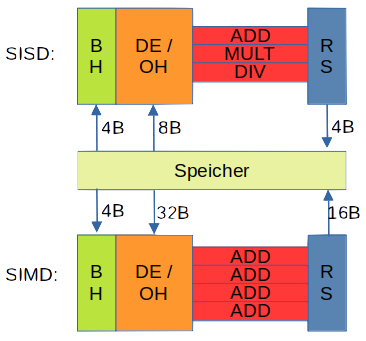
\includegraphics[scale=0.9]{simd.png}
			Bei Grafikkarten (GPUs) wird dieses architekturelle Prinzip auf die Spitze getrieben: Hier haben wir nur ein (oder ein paar wenige) Steuerwerke, die in jedem Takt nur einen (oder ein paar wenige) Operationen holen, und dann auf einer extrem großen Anzahl an Recheneinheiten (im Kontext von GPUs auch Shader genannt) diese Operation für große Datenmengen ausführen.
	\subsection{CUDA Modell}
		\subsubsection{GPU (Graphics Processing Unit)}
			Die Grafikkarte als Ganzes. Ein normaler Rechner besitzt in der Regel eine GPU (manchmal auch 2), oftmals als eigenes Gerät außerhalb der CPU. Günstige Rechner besitzen hingegen GPUs, die direkt mit in der CPU integriert sind (Integrated Graphics). Diese sind aber entsprechend sehr klein und leistungsschwach
		\subsubsection{Streaming Multiprocessor}
			Eine GPU besitzt ein oder mehrere Streaming Multiprocessors (SMs). Dies ist vergleichbar mit dem Konzept von Multicore bei CPUs: Jeder SM arbeitet unabhängig voneinander und kann auch tatsächlich verschiedene Instruktionen ausführen. SMs sind also relativ zueinander nicht SIMD
		\subsubsection{Shader}
			Ein Streaming Multiprocessor besteht aus einer Vielzahl an Shaders (typischerweise ca. 32). Diese Shader innerhalb eines SMs arbeiten nach dem SIMD Prinzip! Sie führen zeitgleich die exakt selbe Instruktion aus, auf unterschiedlichen Daten. Ein Shader beherrscht die absoluten Grundrechenoperationen, z.B. addieren und multiplizieren
		\subsubsection{Special Function Units}
			eder Streaming Multiprocessor besitzt neben den Shadern auch meistens noch 1-2 SFUs. Diese berechnen komplexere Dinge, wie z.B. Sinus oder Kosinus. Da wir davon aber nur sehr wenige haben, funktionieren sie nicht nach dem parallelen SIMD-Prinzip, sondern müssen sequentiell ausgeführt werden. Dies ist natürlich langsam - aber es ist immer noch schneller, als zu sagen, dass die GPU gar keinen Sinus/Kosinus kann und man jedes Mal diese Berechnung (die als Zwischenschritt in einem echten SIMD-Programm vorkommen könnte) an die CPU zu schicken \newline \newline
		\begin{center}
			\textbf{GPU mit 4 SMs, mit jeweils 12 Shadern und 2 FSUs} \newline
			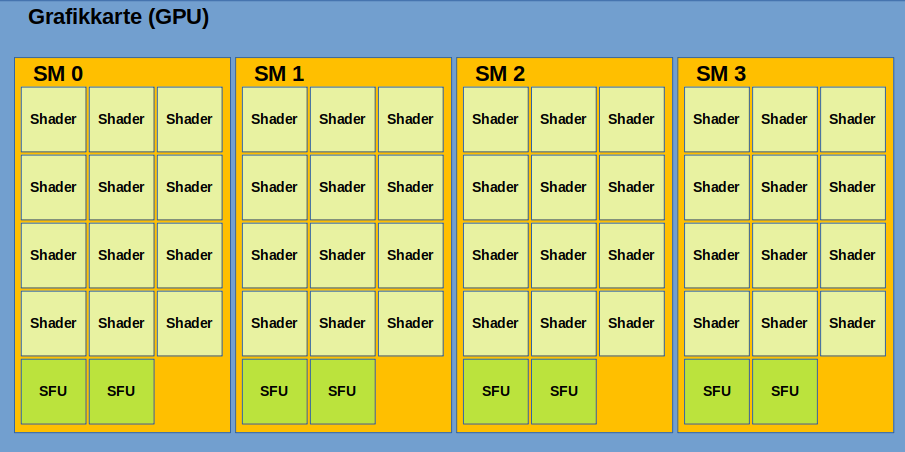
\includegraphics[scale=0.4]{gpu.png}
		\end{center}
	\subsection{CUDA Programmieren}
		Genau wie die Grafikkarten hierarchisch unterteilt ist (GPU -> Streaming Multiprocessor -> Shader) müssen beim CUDA-Modell auch Programmierer*innen ihr Problem unterteilen. Das Gesamtproblem kann man dabei als die gesamte Datenmenge verstehen, die verrechnet werden soll
		\subsubsection{Grid}
			Die gesamte Datenmenge, die von einer Grafikkarte (GPU) verrechnet werden soll, wird als "Grid" bezeichnet. Dies kann eindimensional (z.B. ein Vektor), zweidimensional (z.B. eine Matrix) oder dreidimensional (z.B. 3D Matrizen für 3D Computerspiele) sein
		\subsubsection{Block}
			Das Grid wird wiederum in Blöcke gleicher Größe unterteilt. Auch hier sind bis zu 3 Dimensionen möglich (sinnvollerweise identisch zur Griddimension). Ein Block wird von einem Streaming Multiprocessor bearbeitet	
		\subsubsection{Thread}
			Ein Block besteht wiederum aus mehreren Threads. Ein Thread ist in der Regel für nur ein Datenelement zuständig (theoretisch sind aber auch mehr möglich). Ein Thread wird von einem Shader ausgeführt \newline
		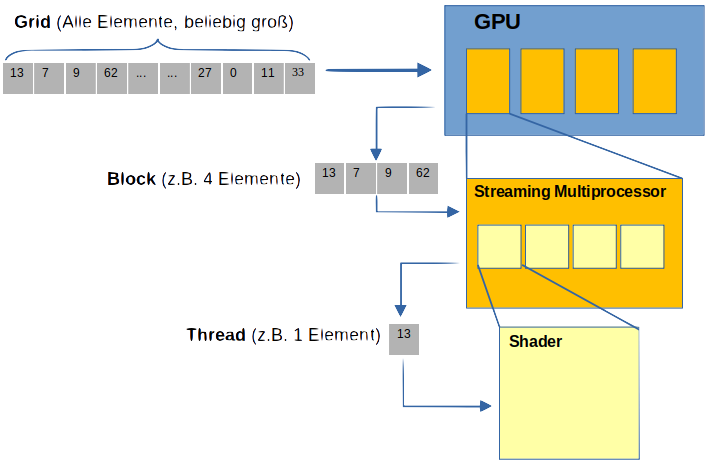
\includegraphics[scale=0.5]{cudamodell.png}
		\subsubsection{Code}
\begin{minted}{c}
__global__ void VectorAdd(float *vectorA, float *vectorB, int size){
	int index = blockIdx.x * blockDim.x * threadIdx.x;
	if (index < size)
		targetVector[index] = vectorA[index] * vectorB[index];	
	}
}
\end{minted}
			Die Funktion erhält als Funktionsargumente die Anfangsadressen der Vektoren  sowie die Gesamtgröße der Vektoren (damit wir nicht versehentlich Werte außerhalb der Vektoren betrachten \newline \newline
			In Zeile 3 bekommt jeder Shader mitgeteilt, für welches Element (bzw. welchen Index innerhalb des Vektors) er zuständig ist: Jeder Streaming Multiprocessor bekommt hierzu dynamisch vom GPU Scheduler einen sogenannten Block-Index (\verb|blockIdx|) zugewiesen, und jeder Shader darin bekommt dynamisch eine sogenannte Thread-ID (\verb|threadIdx|) zugewiesen. Da wir auch festgelegt haben, wie viele Threads es in einem Block gibt (\verb|blockDim|), kann jeder Shader sich dadurch seinen Vektorindex ausrechnen \newline \newline
			Anschließend wird geprüft, ob der Index überhaupt noch innerhalb des Vektors liegt. Wenn das der Fall ist, addieren wir die Werte der beiden Vektoren \verb|vectorA[index]| und \verb|vectorB[index]| zusammen und speichern es wiederum im Zielvektor \verb|targetVector[index]| 
		\subsubsection{Verzweigungen im CPU-Code}
			Bedingte Anweisungen, bei denen nur eine Teilmenge der Shader etwas rechnen soll, werden in der Regel so realisiert, dass durch die Bedingung die jeweils anderen Shader temporär "deaktiviert" werden. Am Ende der Verzweigung werden sie wieder "aktiviert".
			